% !TeX program = pdflatex
\documentclass[tikz,border=8pt]{standalone}
\usepackage{tikz}\usetikzlibrary{angles,quotes}
\definecolor{FigureBlue}{HTML}{2563EB}\definecolor{FigureOrange}{HTML}{EA580C}\definecolor{FigureGreen}{HTML}{16A34A}
\begin{document}
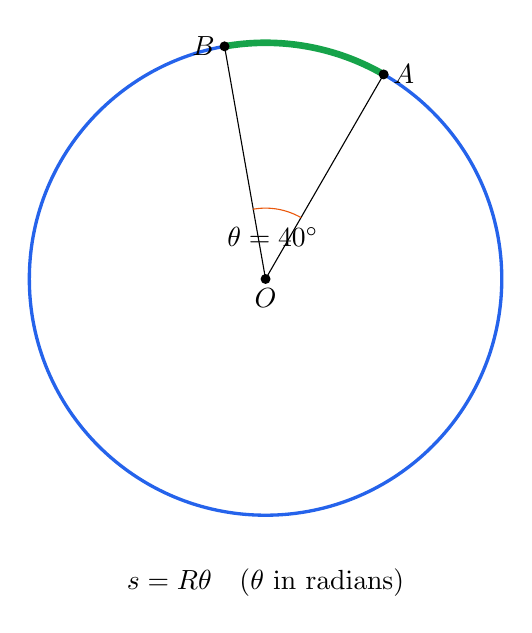
\begin{tikzpicture}[line cap=round]
  \coordinate (O) at (0,0); \coordinate (A) at (60:3); \coordinate (B) at (100:3);
  \draw[FigureBlue,line width=1.2pt] (O) circle (3); \draw (O)--(A) (O)--(B);
  \draw[FigureGreen,line width=2.4pt] (A) arc[start angle=60,end angle=100,radius=3];
  \pic[draw=FigureOrange,angle radius=9mm,"$\theta=40^\circ$"] {angle=A--O--B};
  \fill (O) circle (1.8pt); \fill (A) circle (1.8pt); \fill (B) circle (1.8pt);
  \node[below] at (O) {$O$}; \node[right] at (A) {$A$}; \node[left] at (B) {$B$};
  \node at (0,-3.85) {$s=R\theta\quad(\theta\ \mathrm{in\ radians})$};
\end{tikzpicture}
\end{document}
